\section{球体}\label{sec:球体}

\keyindex{球}{sphere}{}是称为\keyindex{二次曲面}{quadrics}{}——
由$x,y$和$z$的二次多项式描述的通用类型曲面的一种特殊情况。
它是最简单的曲面类型,对光线追踪器很有用,是通用光线相交例程很好的起点。
pbrt支持六种二次曲面:球、\keyindex{圆锥体}{cone}{}、
\keyindex{圆盘}{disk}{}(圆锥的一种特例)、\keyindex{圆柱体}{cylinder}{}、
\keyindex{双曲面}{hyperboloid}{}和\keyindex{抛物面}{paraboloid}{}。

许多曲面能以两种主要方式之一
描述:\keyindex{隐式形式}{implicit form}{}和\keyindex{参数形式}{parametric form}{}。
隐式函数将3D曲面描述为
\begin{align*}
    f(x,y,z)=0\, .
\end{align*}

所有满足该条件的点$(x,y,z)$的集合定义了该曲面。
对于位于原点的单位球体,熟悉的隐式函数是$x^2+y^2+z^2-1=0$。
只有距离原点一单位的点的集合才满足该约束,给出单位球的表面。

许多曲面也能用函数将2D点映射为曲面上的3D点来参数化地描述。
例如,半径为$r$的球体可以描述为2D球面坐标$(\theta,\varphi)$的函数,
其中$\theta$范围是从$0$到$\pi$,$\varphi$范围是从$0$到$2\pi$(\reffig{3.4}):
\begin{align*}
    x & =r\sin\theta\cos\varphi\, , \\
    y & =r\sin\theta\sin\varphi\, , \\
    z & =r\cos\theta\, .
\end{align*}
\begin{figure}[htbp]
    \centering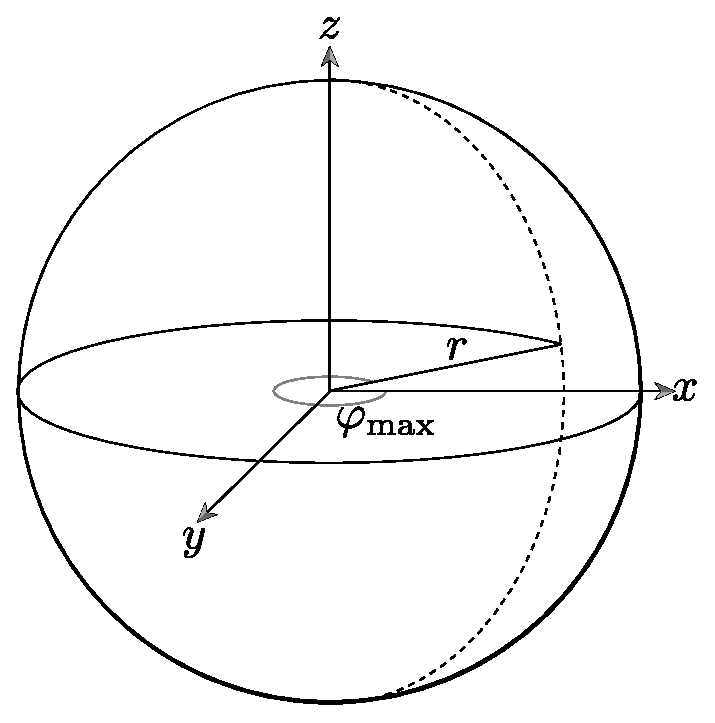
\includegraphics[width=0.5\linewidth]{chap03/Spheresetting.eps}
    \caption{球体形状基本设置。它半径为$r$,球心位于物体空间原点。
        部分球体可以通过指定$\varphi$的最大值描述。}
    \label{fig:3.4}
\end{figure}

我们可以用以下替换将该函数$f(\theta,\varphi)$转换为$[0,1]^2$上的函数$f(u,v)$并
稍微将其一般化以允许部分球体只扫过$\theta\in[\theta_{\min},\theta_{\max}]$和$\varphi\in[0,\varphi_{\max}]$:
\begin{align*}
    \varphi & =u\varphi_{\max}\, ,                              \\
    \theta  & =\theta_{\min}+v(\theta_{\max}-\theta_{\min})\, .
\end{align*}

该形式对纹理贴图特别有用,它能直接用来
将定义在$[0,1]^2$上的纹理映射到球上。
\reffig{3.5}展示了两个球的一张图像;一张网格图像用于展示$(u,v)$参数化。
\begin{figure}[htbp]
    \centering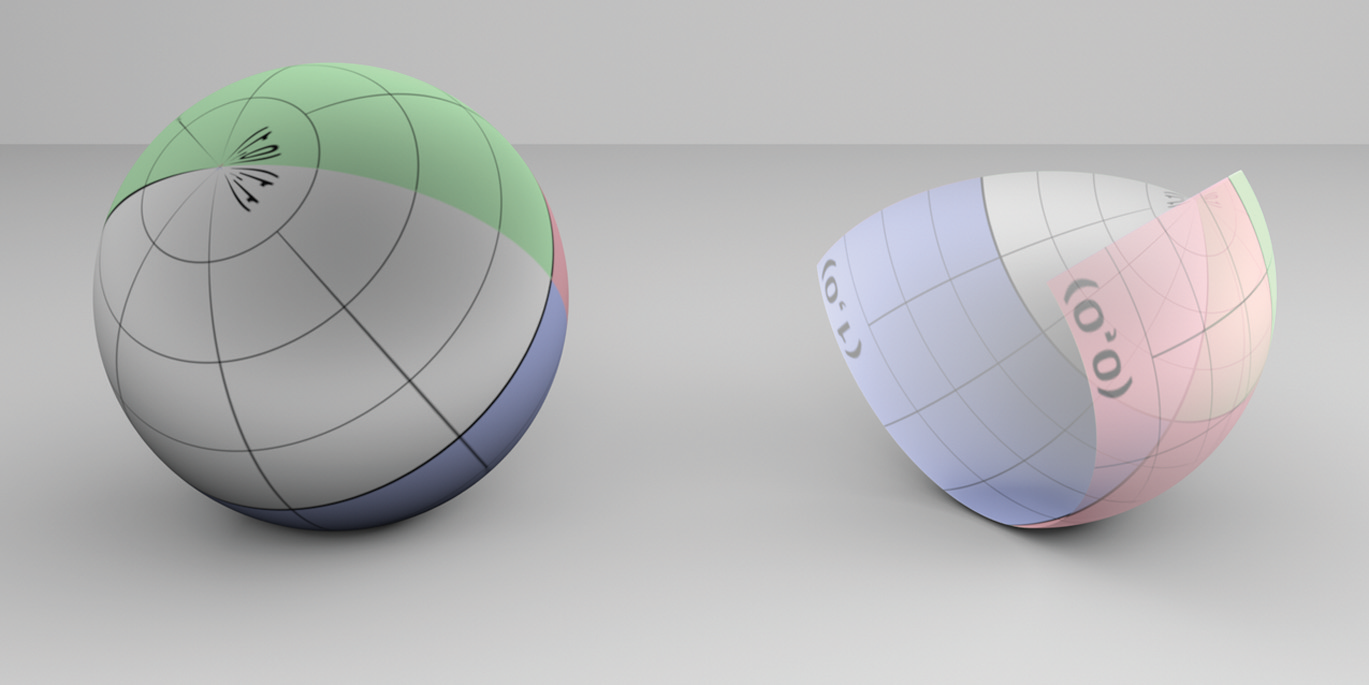
\includegraphics[width=\linewidth]{chap03/twospheres.png}
    \caption{两个球。左边是完整球,右边是部分球($z_{\max}<r$和$\varphi_{\max}<2\pi$)。
        注意纹理贴图用来展示形状$(u,v)$参数化;一极的\protect\keyindex{奇点}{singularity}{}在完整球中可见。}
    \label{fig:3.5}
\end{figure}

当我们描述球形状的实现时,我们将同时利用形状的隐式和参数化描述,
这取决于哪种方式能更自然地解决我们面临的特定问题。

类\refvar{Sphere}{}表示球心在物体空间原点的球体。
其实现在\href{https://github.com/mmp/pbrt-v3/tree/master/src/shapes/sphere.h}{\ttfamily shapes/sphere.h}
和\href{https://github.com/mmp/pbrt-v3/tree/master/src/shapes/sphere.cpp}{\ttfamily shapes/sphere.cpp}文件中。
\begin{lstlisting}
`\initcode{Sphere Declarations}{=}`
class `\initvar{Sphere}{}` : public `\refvar{Shape}{}` {
public:
    `\refcode{Sphere Public Methods}{}`
private:
    `\refcode{Sphere Private Data}{}`
};
\end{lstlisting}

为了在场景中别处放置球体,用户在输入文件里指定球体时必须施加合适的变换。
它同时接收物体到世界和世界到物体的变换作为参数给构造函数,
并将它们传给父类\refvar{Shape}{}的构造函数。

球的半径可以是任意正值,且球的范围可用两种方式截断。
第一,设置最小和最大$z$值;球体分别位于这些平面之下和之上的部分会被切除。
第二,在球面坐标中考虑球的参数化,可设置最大的$\varphi$值。
球体的$\varphi$值扫过从$0$到给定$\varphi_{\max}$的范围,
这样超出$\varphi_{\max}$的$\varphi$值对应的球体部分也被移除。
\begin{lstlisting}
`\initcode{Sphere Public Methods}{=}`
`\refvar{Sphere}{}`(const `\refvar{Transform}{}` *ObjectToWorld, const `\refvar{Transform}{}` *WorldToObject,
       bool reverseOrientation, `\refvar{Float}{}` radius, `\refvar{Float}{}` zMin, `\refvar{Float}{}` zMax,
       `\refvar{Float}{}` phiMax)
    : `\refvar{Shape}{}`(ObjectToWorld, WorldToObject, reverseOrientation),
      `\refvar[Sphere::radius]{radius}{}`(radius), `\refvar[Sphere::zMin]{zMin}{}`(`\refvar{Clamp}{}`(std::min(zMin, zMax), -radius, radius)),
      `\refvar[Sphere::zMax]{zMax}{}`(`\refvar{Clamp}{}`(std::max(zMin, zMax), -radius, radius)),
      `\refvar[Sphere::thetaMin]{thetaMin}{}`(std::acos(`\refvar{Clamp}{}`(zMin / radius, -1, 1))),
      `\refvar[Sphere::thetaMax]{thetaMax}{}`(std::acos(`\refvar{Clamp}{}`(zMax / radius, -1, 1))),
      `\refvar[Sphere::phiMax]{phiMax}{}`(`\refvar{Radians}{}`(`\refvar{Clamp}{}`(phiMax, 0, 360))) { }
\end{lstlisting}
\begin{lstlisting}
`\initcode{Sphere Private Data}{=}`
const `\refvar{Float}{}` `\initvar[Sphere::radius]{radius}{}`;
const `\refvar{Float}{}` `\initvar[Sphere::zMin]{zMin}{}`, `\initvar[Sphere::zMax]{zMax}{}`;
const `\refvar{Float}{}` `\initvar[Sphere::thetaMin]{thetaMin}{}`, `\initvar[Sphere::thetaMax]{thetaMax}{}`, `\initvar[Sphere::phiMax]{phiMax}{}`;
\end{lstlisting}

\subsection{边界}\label{sub:边界2}
计算球体的物体空间边界框很简单。
当要渲染的部分少于整个球体时,这里的实现使用用户提供的$z_{\min}$和$z_{\max}$值来缩紧边界。
然而,当$\varphi_{\max}$少于$\displaystyle\frac{3\pi}{2}$时它并不做额外工作计算更紧的边界框。
该改进留作习题。
\begin{lstlisting}
`\initcode{Sphere Method Definitions}{=}\initnext{SphereMethodDefinitions}`
`\refvar{Bounds3f}{}` `\refvar{Sphere}{}`::`\initvar[Sphere::ObjectBound]{\refvar{ObjectBound}{}}{}`() const {
    return `\refvar{Bounds3f}{}`(`\refvar{Point3f}{}`(-`\refvar[Sphere::radius]{radius}{}`, -`\refvar[Sphere::radius]{radius}{}`, `\refvar[Sphere::zMin]{zMin}{}`),
                    `\refvar{Point3f}{}`( `\refvar[Sphere::radius]{radius}{}`,  `\refvar[Sphere::radius]{radius}{}`, `\refvar[Sphere::zMax]{zMax}{}`));
}
\end{lstlisting}

\subsection{相交测试}\label{sub:相交测试2}
推导光线-球体相交测试的任务被球心位于原点的事实简化了。
然而如果球已被变换到世界空间的另一位置,
则光线与球相交前需要用世界到物体的变换来变到物体空间。
有了物体空间的光线,就能在物体空间执行相交计算了
\footnote{这是计算机图形学的经典主题。
    通过把问题转换为特定受限的情况,就可能更简单高效地做相交测试:
    即因为球总是在$(0,0,0)$,方程的许多项就消掉了。
    这不会失去一般性,因为对于其他位置的球体,适当平移光线即可。}。

下列代码片展示了整个相交方法:
\begin{lstlisting}
`\refcode{Sphere Method Definitions}{+=}\lastnext{SphereMethodDefinitions}`
bool `\refvar{Sphere}{}`::`\initvar[Sphere::Intersect]{\refvar[Shape::Intersect]{Intersect}{}}{}`(const `\refvar{Ray}{}` &r, `\refvar{Float}{}` *tHit,
        `\refvar{SurfaceInteraction}{}` *isect, bool testAlphaTexture) const {
    `\refvar{Float}{}` phi;
    `\refvar{Point3f}{}` pHit;
    `\refcode{Transform Ray to object space}{}`
    `\refcode{Compute quadratic sphere coefficients}{}`
    `\refcode{Solve quadratic equation for t values}{}`
    `\refcode{Compute sphere hit position and $\varphi$}{}`
    `\refcode{Test sphere intersection against clipping parameters}{}`
    `\refcode{Find parametric representation of sphere hit}{}`
    `\refcode{Compute error bounds for sphere intersection}{}`
    `\refcode{Initialize SurfaceInteraction from parametric information}{}`
    `\refcode{Update tHit for quadric intersection}{}`
    return true;
}
\end{lstlisting}

首先,所给世界空间光线被变换到球的物体空间。
相交测试的剩余部分将在那个坐标系统内进行。
{\ttfamily oErr}和{\ttfamily dErr}变量分别定界
在变换射线端点和方向时因为施加变换而引入的浮点舍入误差
(更多关于浮点算术和其对于准确光线相交计算实现的更多信息见\refsec{控制舍入误差})。
\begin{lstlisting}
`\initcode{Transform Ray to object space}{=}`
`\refvar{Vector3f}{}` oErr, dErr;
`\refvar{Ray}{}` ray = (*`\refvar{WorldToObject}{}`)(r, &oErr, &dErr);
\end{lstlisting}

如果球心在原点,半径为$r$,则其隐式表示是
\begin{align*}
    x^2+y^2+z^2-r^2=0\, .
\end{align*}

通过将\refeq{2.3}中射线的参数表示代入隐式球方程,我们有
\begin{align*}
    (o_x+td_x)^2+(o_y+td_y)^2+(o_z+td_z)^2=r^2\, .
\end{align*}

注意该方程除了$t$的所有元素都是已知量。
使方程成立的$t$值给出了光线上使隐式球方程成立的参数化位置,
即沿光线与球相交的点。
我们可以展开该方程并整理系数得到$t$的一般二次方程,
\begin{align*}
    at^2+bt+c=0\, ,
\end{align*}
其中\footnote{一些光线追踪器要求规范化射线方向向量,即$a=1$。
    然而如果调用者忘记规范化射线方向则会导致微妙错误。
    当然,该错误可以通过在射线构造函数内规范化方向来避免,
    但这在提供的方向\emph{已经}规范化时会浪费精力。
    为了避免这无用的复杂性,pbrt没有在相交例程中坚持向量规范化。
    这特别有用,因为它减少了将射线变换到物体空间所需的计算量,即不需要规范化。}
\begin{align*}
    a & =d_x^2+d_y^2+d_z^2\, ,       \\
    b & =2(d_xo_x+d_yo_y+d_zo_z)\, , \\
    c & =o_x^2+o_y^2+o_z^2-r^2\, .
\end{align*}

该结果可以直接翻译为源码片。注意在该代码中,
类\refvar{EFloat}{}的而不是\refvar{Float}{}
的实例用于表示浮点值。\refvar{EFloat}{}跟踪累积的浮点舍入误差;
\refsec{控制舍入误差}将讨论它的使用。
至于现在,阅读时可以认为它和\refvar{Float}{}等价。
\begin{lstlisting}
`\initcode{Compute quadratic sphere coefficients}{=}`
`\refcode{Initialize EFloat ray coordinate values}{}`
`\refvar{EFloat}{}` a = dx * dx + dy * dy + dz * dz;
`\refvar{EFloat}{}` b = 2 * (dx * ox + dy * oy + dz * oz);
`\refvar{EFloat}{}` c = ox * ox + oy * oy + oz * oz - `\refvar{EFloat}{}`(`\refvar[Sphere::radius]{radius}{}`) * `\refvar{EFloat}{}`(`\refvar[Sphere::radius]{radius}{}`);
\end{lstlisting}

相交测试用的射线端点和方向值由将射线变换到物体空间的浮点误差界初始化。
\begin{lstlisting}
`\initcode{Initialize EFloat ray coordinate values}{=}`
`\refvar{EFloat}{}` ox(ray.o.x, oErr.x), oy(ray.o.y, oErr.y), oz(ray.o.z, oErr.z);
`\refvar{EFloat}{}` dx(ray.d.x, dErr.x), dy(ray.d.y, dErr.y), dz(ray.d.z, dErr.z);
\end{lstlisting}

二次方程有两个可能的解,给出光线交于球体的零、一或两个非虚数$t$值。
\begin{lstlisting}
`\initcode{Solve quadratic equation for t values}{=}`
`\refvar{EFloat}{}` t0, t1;
if (!`\refvar{Quadratic}{}`(a, b, c, &t0, &t1))
    return false;
`\refcode{Check quadric shape t0 and t1 for nearest intersection}{}`
\end{lstlisting}

实用函数\refvar{Quadratic}{}求解二次方程,
如果没有实数解就返回{\ttfamily false},
如果有则返回{\ttfamily true}并适当设置{\ttfamily t0}和{\ttfamily t1}。
稍后将在\refsub{求解二次方程}\sidenote{译者注:原文此处似乎链接章节错误,已修正。}定义它,
我们会讨论怎样用浮点算术稳定地实现它。

算得的参数化距离{\ttfamily t0}和{\ttfamily t1}跟踪了
原始射线参数的误差和\refvar{Quadratic}{}内累积的误差造成的不确定性;
不确定性区间范围的下界和上界可以使用方法\refvar[LowerBound]{EFloat::LowerBound}{()}和
\refvar[UpperBound]{EFloat::UpperBound}{()}获取。

代码片\refcode{Check quadric shape t0 and t1 for nearest intersection}{}取
两个相交值并确定如果有的话哪一个是最近的有效相交处。
对于有效的相交处,其值必须大于零且小于{\ttfamily ray.\refvar{tMax}{}}。
下列代码使用类\refvar{EFloat}{}提供的误差区间并只接受
明确在范围$(0,$\refvar{tMax}{}$)$内的相交处。

因为$t_0$保证小于或等于$t_1$(且$0$小于\refvar{tMax}{}),
则如果$t_0$大于\refvar{tMax}{}或$t_1$小于$0$,
那么两个相交处都一定超出了考虑范围。
否则,$t_0$是暂时的命中$t$值。
但它可能小于$0$,这时我们忽略它并尝试$t_1$。
如果也超出范围,我们就没有有效相交处。
如果有一个相交处,则初始化{\ttfamily tShapeHit}来保存该相交处的参数$t$值。
\begin{lstlisting}
`\initcode{Check quadric shape t0 and t1 for nearest intersection}{=}`
if (t0.`\refvar{UpperBound}{}`() > ray.`\refvar{tMax}{}` || t1.`\refvar{LowerBound}{}`() <= 0)
    return false;
`\refvar{EFloat}{}` tShapeHit = t0;
if (tShapeHit.`\refvar{LowerBound}{}`() <= 0) {
    tShapeHit = t1;
    if (tShapeHit.`\refvar{UpperBound}{}`() > ray.`\refvar{tMax}{}`)
        return false;
}
\end{lstlisting}
有了射线与完整球体相交的参数距离,
就能按沿射线的偏移量计算交点{\ttfamily pHit}。

接下来需要处理带有截断$z$或$\varphi$范围的部分球体——
必须忽略与截去区域的相交。
实现从计算命中点的$\varphi$值开始。使用球的参数化表示,
\begin{align*}
    \frac{y}{x}=\frac{r\sin\theta\sin\varphi}{r\sin\theta\cos\varphi}=\tan\varphi\, ,
\end{align*}
所以$\displaystyle\varphi=\arctan\frac{y}{x}$。
为了符合球的原始定义,需要将标准库函数{\ttfamily std::atan()}的
结果重新映射为$0$到$2\pi$的值。
\begin{lstlisting}
`\initcode{Compute sphere hit position and $\varphi$}{=}`
pHit = ray((`\refvar{Float}{}`)tShapeHit);
`\refcode{Refine sphere intersection point}{}`
if (pHit.x == 0 && pHit.y == 0) pHit.x = 1e-5f * `\refvar[Sphere::radius]{radius}{}`;
phi = std::atan2(pHit.y, pHit.x);
if (phi < 0) phi += 2 * `\refvar{Pi}{}`;
\end{lstlisting}

由于浮点精度限制,算得的该交点{\ttfamily pHit}可能位于实际球体表面的一侧;
定义于\refsub{定界交点误差}的
代码片\refcode{Refine sphere intersection point}{}会提升该值精度。

现在可以针对$z$和$\varphi$指定的最小值和最大值测试命中点了。
一个细节是如果$z$范围包括了整个球体则跳过$z$测试非常重要;
算得的值{\ttfamily pHit.z}可能因为浮点舍入超出$z$范围一点点,
所以我们应该只在用户希望球体是部分不完整时才执行该测试。
如果$t_0$相交处实际无效,例程就再次尝试$t_1$。
\begin{lstlisting}
`\initcode{Test sphere intersection against clipping parameters}{=}`
if ((`\refvar[Sphere::zMin]{zMin}{}` > -`\refvar[Sphere::radius]{radius}{}` && pHit.z < `\refvar[Sphere::zMin]{zMin}{}`) ||
    (`\refvar[Sphere::zMax]{zMax}{}` <  `\refvar[Sphere::radius]{radius}{}` && pHit.z > `\refvar[Sphere::zMax]{zMax}{}`) || phi > `\refvar[Sphere::phiMax]{phiMax}{}`) {
    if (tShapeHit == t1) return false;
    if (t1.`\refvar{UpperBound}{}`() > ray.`\refvar{tMax}{}`) return false;
    tShapeHit = t1;
    `\refcode{Compute sphere hit position and $\varphi$}{}`
    if ((`\refvar[Sphere::zMin]{zMin}{}` > -`\refvar[Sphere::radius]{radius}{}` && pHit.z < `\refvar[Sphere::zMin]{zMin}{}`) ||
        (`\refvar[Sphere::zMax]{zMax}{}` <  `\refvar[Sphere::radius]{radius}{}` && pHit.z > `\refvar[Sphere::zMax]{zMax}{}`) || phi > `\refvar[Sphere::phiMax]{phiMax}{}`)
        return false;
}
\end{lstlisting}

在例程中的此处,光线一定命中了球体。
接下来方法分别通过缩放之前计算的$\varphi$值来为命中点计算在0到1之间的$u$值,
并基于所给球体的$\theta$值范围通过为命中点计算0到1的$\theta$值来计算$v$值
\sidenote{译者注:这句话太绕了,我投降,请大佬赐教怎么翻译。
    看不懂没关系,去翻翻前面$u,v$与$\varphi,\theta$的关系你就懂了。}。
然后它再求位置的参数化偏导数$\displaystyle\frac{\partial \bm p}{\partial u}$和
$\displaystyle\frac{\partial \bm p}{\partial v}$以及
曲面法线的$\displaystyle\frac{\partial \bm n}{\partial u}$和
$\displaystyle\frac{\partial \bm n}{\partial v}$。
\begin{lstlisting}
`\initcode{Find parametric representation of sphere hit}{=}`
`\refvar{Float}{}` u = phi / `\refvar[Sphere::phiMax]{phiMax}{}`;
`\refvar{Float}{}` theta = std::acos(`\refvar{Clamp}{}`(pHit.z / `\refvar[Sphere::radius]{radius}{}`, -1, 1));
`\refvar{Float}{}` v = (theta - `\refvar[Sphere::thetaMin]{thetaMin}{}`) / (`\refvar[Sphere::thetaMax]{thetaMax}{}` - `\refvar[Sphere::thetaMin]{thetaMin}{}`);
`\refcode{Compute sphere $\partial$p/$\partial$u and $\partial$p/$\partial$v}{}`
`\refcode{Compute sphere $\partial$n/$\partial$u and $\partial$n/$\partial$v}{}`
\end{lstlisting}

计算球上一点的偏导数是个代数小习题。
这里我们将展示怎样计算$\displaystyle\frac{\partial \bm p}{\partial u}$的$x$分量,
$\displaystyle\frac{\partial p_x}{\partial u}$;
其他分量解法相同。使用球的参数化定义,我们有\sidenote{译者注:这里$p_x$与$x$含义相同,以此类推。}
\begin{align*}
    x                               & =r\sin\theta\cos\varphi\, ,                          \\
    \frac{\partial p_x}{\partial u} & =\frac{\partial}{\partial u}(r\sin\theta\cos\varphi) \\
                                    & =r\sin\theta\frac{\partial\cos\varphi}{\partial u}   \\
                                    & =-r\varphi_{\max}\sin\theta\sin\varphi\, .
\end{align*}

基于球$y$坐标的参数化定义进行代换,可以简化为
\begin{align*}
    \frac{\partial p_x}{\partial u}=-\varphi_{\max}y\, .
\end{align*}
同样
\begin{align*}
    \frac{\partial p_y}{\partial u}=\varphi_{\max}x\, ,
\end{align*}
以及
\begin{align*}
    \frac{\partial p_z}{\partial u}=0\, .
\end{align*}

同样过程求得$\displaystyle\frac{\partial \bm p}{\partial v}$,完整结果为
\begin{align*}
    \frac{\partial \bm p}{\partial u} & =(-\varphi_{\max}y,\varphi_{\max}x,0)\, ,                                  \\
    \frac{\partial \bm p}{\partial v} & =(\theta_{\max}-\theta_{\min})(z\cos\varphi,z\sin\varphi,-r\sin\theta)\, .
\end{align*}
\begin{lstlisting}
`\initcode{Compute sphere $\partial$p/$\partial$u and $\partial$p/$\partial$v}{=}`
`\refvar{Float}{}` zRadius = std::sqrt(pHit.x * pHit.x + pHit.y * pHit.y);
`\refvar{Float}{}` invZRadius = 1 / zRadius;
`\refvar{Float}{}` cosPhi = pHit.x * invZRadius;
`\refvar{Float}{}` sinPhi = pHit.y * invZRadius;
`\refvar{Vector3f}{}` dpdu(-`\refvar[Sphere::phiMax]{phiMax}{}` * pHit.y, `\refvar[Sphere::phiMax]{phiMax}{}` * pHit.x, 0);
`\refvar{Vector3f}{}` dpdv = (`\refvar[Sphere::thetaMax]{thetaMax}{}` - `\refvar[Sphere::thetaMin]{thetaMin}{}`) *
    `\refvar{Vector3f}{}`(pHit.z * cosPhi, pHit.z * sinPhi,
             -`\refvar[Sphere::radius]{radius}{}` * std::sin(theta));
\end{lstlisting}

\subsection{法向量的偏导数}\label{sub:法向量的偏导数}
\begin{remark}
    本节含有高级内容,第一次阅读时可以跳过。
\end{remark}

当我们沿表面在$u$和$v$方向移动时,确定法线是怎样变化的也很有用。
例如,第\refchap{纹理}的抗锯齿技术就依赖于该信息来消除物体曲面上反射可见的纹理锯齿。
法线的微分变化量$\displaystyle\frac{\partial \bm n}{\partial u}$和
$\displaystyle\frac{\partial \bm n}{\partial v}$由微分几何学
的\keyindex{微分几何基础}{Weingarten equations}{}给出
\sidenote{译者注:得名于德国数学家Julius Weingarten。
    相关简要推导详见译者整理补充的\refsec{微分几何基础}。
    注意该公式其实隐含了对$\bm n$的规范化要求。
    下面所提的第一基本形式、第二基本形式也是微分几何学中的概念。}:
\begin{align*}
    \frac{\partial \bm n}{\partial u} & =\frac{fF-eG}{EG-F^2}\frac{\partial \bm p}{\partial u}+\frac{eF-fE}{EG-F^2}\frac{\partial \bm p}{\partial v}\, , \\
    \frac{\partial \bm n}{\partial v} & =\frac{gF-fG}{EG-F^2}\frac{\partial \bm p}{\partial u}+\frac{fF-gE}{EG-F^2}\frac{\partial \bm p}{\partial v}\, ,
\end{align*}
其中$E,F$和$G$是\keyindex{第一基本形式}{the first fundamental form}{}的系数,即
\begin{align*}
    E & =\left|\frac{\partial \bm p}{\partial u}\right|^2\, ,                                     \\
    F & =\left(\frac{\partial \bm p}{\partial u}\cdot\frac{\partial \bm p}{\partial v}\right)\, , \\
    G & =\left|\frac{\partial \bm p}{\partial v}\right|^2\, .
\end{align*}

它们可以利用之前算得的$\displaystyle\frac{\partial \bm p}{\partial u}$和$\displaystyle\frac{\partial \bm p}{\partial v}$轻松算出。
$e,f$和$g$是\keyindex{第二基本形式}{the second fundamental form}{}的系数,
\begin{align*}
    e & =\left(\bm n\cdot\frac{\partial^2\bm p}{\partial u^2}\right)\, ,         \\
    f & =\left(\bm n\cdot\frac{\partial^2\bm p}{\partial u\partial v}\right)\, , \\
    g & =\left(\bm n\cdot\frac{\partial^2\bm p}{\partial v^2}\right)\, .
\end{align*}

两个基本形式刻画了曲面的基本度量属性,包括距离、角度和\keyindex{曲率}{curvature}{}的概念;
细节详见微分几何教材例如\citet{gray2017modern}
\sidenote{译者注:此处引用文献改为了新版。}。
为了求$e,f$和$g$,需要计算二阶偏导数$\displaystyle\frac{\partial^2\bm p}{\partial u^2}$等。

对于球体,可以算得二阶导数为:
\begin{align*}
    \frac{\partial^2\bm p}{\partial u^2}         & =-\varphi_{\max}^2(x,y,0)\, ,                                                 \\
    \frac{\partial^2\bm p}{\partial u\partial v} & =(\theta_{\max}-\theta_{\min})z\varphi_{\max}(-\sin\varphi,\cos\varphi,0)\, , \\
    \frac{\partial^2\bm p}{\partial v^2}         & =-(\theta_{\max}-\theta_{\min})^2(x,y,z)\, .
\end{align*}
\begin{lstlisting}
`\initcode{Compute sphere $\partial$n/$\partial$u and $\partial$n/$\partial$v}{=}`
`\refvar{Vector3f}{}` d2Pduu = -`\refvar[Sphere::phiMax]{phiMax}{}` * `\refvar[Sphere::phiMax]{phiMax}{}` * `\refvar{Vector3f}{}`(pHit.x, pHit.y, 0);
`\refvar{Vector3f}{}` d2Pduv = (`\refvar[Sphere::thetaMax]{thetaMax}{}` - `\refvar[Sphere::thetaMin]{thetaMin}{}`) * pHit.z * `\refvar[Sphere::phiMax]{phiMax}{}` *
                  `\refvar{Vector3f}{}`(-sinPhi, cosPhi, 0.);
`\refvar{Vector3f}{}` d2Pdvv = -(`\refvar[Sphere::thetaMax]{thetaMax}{}` - `\refvar[Sphere::thetaMin]{thetaMin}{}`) * (`\refvar[Sphere::thetaMax]{thetaMax}{}` - `\refvar[Sphere::thetaMin]{thetaMin}{}`) *
                  `\refvar{Vector3f}{}`(pHit.x, pHit.y, pHit.z);
`\refcode{Compute coefficients for fundamental forms}{}`
`\refcode{Compute $\partial$n/$\partial$u and $\partial$n/$\partial$v from fundamental form coefficients}{}`
\end{lstlisting}
\begin{lstlisting}
`\initcode{Compute coefficients for fundamental forms}{=}`
`\refvar{Float}{}` E = `\refvar{Dot}{}`(dpdu, dpdu);
`\refvar{Float}{}` F = `\refvar{Dot}{}`(dpdu, dpdv);
`\refvar{Float}{}` G = `\refvar{Dot}{}`(dpdv, dpdv);
`\refvar{Vector3f}{}` N = `\refvar{Normalize}{}`(`\refvar{Cross}{}`(dpdu, dpdv));
`\refvar{Float}{}` e = `\refvar{Dot}{}`(N, d2Pduu);
`\refvar{Float}{}` f = `\refvar{Dot}{}`(N, d2Pduv);
`\refvar{Float}{}` g = `\refvar{Dot}{}`(N, d2Pdvv);
\end{lstlisting}
\begin{lstlisting}
`\initcode{Compute $\partial$n/$\partial$u and $\partial$n/$\partial$v from fundamental form coefficients}{=}`
`\refvar{Float}{}` invEGF2 = 1 / (E * G - F * F);
`\refvar{Normal3f}{}` dndu = `\refvar{Normal3f}{}`((f * F - e * G) * invEGF2 * dpdu + 
                         (e * F - f * E) * invEGF2 * dpdv);
`\refvar{Normal3f}{}` dndv = `\refvar{Normal3f}{}`((g * F - f * G) * invEGF2 * dpdu + 
                         (f * F - g * E) * invEGF2 * dpdv);
\end{lstlisting}

\subsection{SurfaceInteraction 初始化}
计算了曲面参数化和所有相关偏导数后,
可以用该相交处的几何信息初始化结构\refvar{SurfaceInteraction}{}了。
传给\refvar{SurfaceInteraction}{}构造函数的\refvar{pError}{}值
定界了算得的点{\ttfamily pHit}中的舍入误差。
它在稍后于\refsub{定界交点误差}定义的代码片\refcode{Compute error bounds for sphere intersection}{}中初始化。
\begin{lstlisting}
`\initcode{Initialize SurfaceInteraction from parametric information}{=}`
*isect = (*`\refvar{ObjectToWorld}{}`)(
    `\refvar{SurfaceInteraction}{}`(pHit, `\refvar{pError}{}`, `\refvar{Point2f}{}`(u, v), -ray.`\refvar[Ray::d]{d}{}`, dpdu, dpdv,
                       dndu, dndv, ray.`\refvar[Ray::time]{time}{}`, this));
\end{lstlisting}

因为有相交处,已存于{\ttfamily tShapeHit}的光线上的命中参数距离将更新
方法\refvar[Shape::Intersect]{Intersect}{}的参数{\ttfamily tHit}。
如果可能的命中点比已有的相交处更远,则更新{\ttfamily *tHit}能让后续相交测试提前终止。
\begin{lstlisting}
`\initcode{Update tHit for quadric intersection}{=}`
*tHit = (`\refvar{Float}{}`)tShapeHit;
\end{lstlisting}

这里自然会问道:“世界到物体变换对于返回正确的参数距离有何影响呢?”
确实,相交方法已经为物体空间射线求得到相交处的参数距离,
它可能已被平移、旋转、缩放,甚至是从世界空间变换来的。
然而,可以证明在物体空间内到相交处的参数距离正好等于
把射线留在世界空间内并在那里求相交后得到的距离,
因此,{\ttfamily *tHit}可以直接设置。
注意如果物体空间射线的方向在变换后被规范化,那就不是这种情况了,
会需要一个与未规范化射线的长度相关的校正因子。
这是变换后不规范化物体空间射线方向向量的另一个动机。

\refvar{Sphere::IntersectP}{()}例程几乎和\refvar{Sphere::Intersect}{()}一样,
但它不初始化结构\refvar{SurfaceInteraction}{}。
因为方法\refvar[Shape::Intersect]{Intersect}{}和\refvar[Shape::IntersectP]{IntersectP}{()}总是如此接近,
接下来我们不再为剩余形状展示\refvar[Shape::IntersectP]{IntersectP}{()}。
\begin{lstlisting}
`\refcode{Sphere Method Definitions}{+=}\lastnext{SphereMethodDefinitions}`
bool `\refvar{Sphere}{}`::`\initvar[Sphere::IntersectP]{\refvar[Shape::IntersectP]{IntersectP}{}}{}`(const `\refvar{Ray}{}` &r, bool testAlphaTexture) const {
    `\refvar{Float}{}` phi;
    `\refvar{Point3f}{}` pHit;
    `\refcode{Transform Ray to object space}{}`
    `\refcode{Compute quadratic sphere coefficients}{}`
    `\refcode{Solve quadratic equation for t values}{}`
    `\refcode{Compute sphere hit position and $\varphi$}{}`
    `\refcode{Test sphere intersection against clipping parameters}{}`
    return true;
}
\end{lstlisting}

\subsection{表面积}\label{sub:表面积2}
为了计算二次曲面的表面积,我们使用\keyindex{积分学}{integral calculus}{}的标准公式。
如果定义于$x=a$到$x=b$的\keyindex{曲线}{curve}{}$y=f(x)$绕$x$轴旋转,
则所得扫掠曲面的表面积为
\begin{align*}
    2\pi\int_a^b{f(x)\sqrt{1+(f'(x))^2}\mathrm{d}x}\, ,
\end{align*}
其中$f'(x)$表示导数$\displaystyle\frac{\mathrm{d}f}{\mathrm{d}x}$。
因为我们大多数的旋转表面都只是绕轴部分扫掠的,所以我们替代使用公式
\begin{align*}
    \varphi_{\max}\int_a^b{f(x)\sqrt{1+(f'(x))^2}\mathrm{d}x}\, .
\end{align*}

球面是\keyindex{圆弧}{circular arc}{}旋转的曲面。
沿球体$z$轴定义轮廓曲线的函数是
\begin{align*}
    f(z)=\sqrt{r^2-z^2}\, ,
\end{align*}
并且其导数为
\begin{align*}
    f'(z)=-\frac{z}{\sqrt{r^2-z^2}}\, .
\end{align*}

回想球体在$z_{\min}$和$z_{\max}$处被裁剪。因此表面积为
\begin{align*}
    A & =\varphi_{\max}\int_{z_{\min}}^{z_{\max}}{\sqrt{r^2-z^2}\sqrt{1+\frac{z^2}{r^2-z^2}}\mathrm{d}z} \\
      & =\varphi_{\max}\int_{z_{\min}}^{z_{\max}}{\sqrt{r^2-z^2+z^2}\mathrm{d}z}                         \\
      & =\varphi_{\max}\int_{z_{\min}}^{z_{\max}}{r\mathrm{d}z}                                          \\
      & =\varphi_{\max}r(z_{\max}-z_{\min})\, .
\end{align*}

对于完整球体$\varphi_{\max}=2\pi$,$z_{\min}=-r$且$z_{\max}=r$,
所以我们有标准公式$A=4\pi r^2$,确认该公式有意义。
\begin{lstlisting}
`\refcode{Sphere Method Definitions}{+=}\lastnext{SphereMethodDefinitions}`
`\refvar{Float}{}` `\refvar{Sphere}{}`::`\initvar[Sphere::Area]{\refvar[Shape::Area]{Area}{}}{}`() const {
    return `\refvar[Sphere::phiMax]{phiMax}{}` * `\refvar[Sphere::radius]{radius}{}` * (`\refvar[Sphere::zMax]{zMax}{}` - `\refvar[Sphere::zMin]{zMin}{}`);
}
\end{lstlisting}